\documentclass{csse4400}

\usepackage{tikz}
\usetikzlibrary{fit}

\usepackage{caption}
\usepackage{subcaption}

\usepackage{languages}

\title{Docker}
\author{Brae Webb}

\date{{\color{red} The Future}}
\begin{document}

\makecover

\maketitle

\section{Introduction}
As developers, we often find ourselves relying on some magical tools and technologies.
Version control, operating systems, databases, and containers, to name a few.
If you are not yet acquainted with containers, and more specifically, docker, you soon will be.
Over the past decade docker has enabled some truly fanciful architectures and developer workflows.
Docker is the proposed solution to the age-old programmer proverb, ``it works on my machine!''.
However, before we get swept up by a snake-oil salespitch, let's see how docker actually works to learn what it is, and what it is not.

\section{History and Fundamentals}
Relative to other tools in the magical suite, docker is new on the scene.
Docker was first made available publicly in 2013 at PyCon.\footnote{\url{https://www.youtube.com/watch?v=wW9CAH9nSLs}}
Pitched to deliver the isolation benefits of Virtual Machines (VMs) while maintaining efficient execution.
Virtual machines themselves are a much older invention, dating back to the 1960s, around the time that UQ was having it's first computer installed%
.\footnote{\url{https://www.youtube.com/watch?v=DB1Y4GrfrZk}}
The concept of a virtual machine, unlike its implementation, is straight-forward --- use software to simulate hardware.
From there, one can install an operating system on the simulated hardware and start using a completely isolated, completely new computer without any additional hardware.
Of course, this process puts great strain on the real hardware and as such, VMs are deployed sparingly.

\begin{figure}[h]
\centering
\begin{subfigure}[b]{0.45\textwidth}
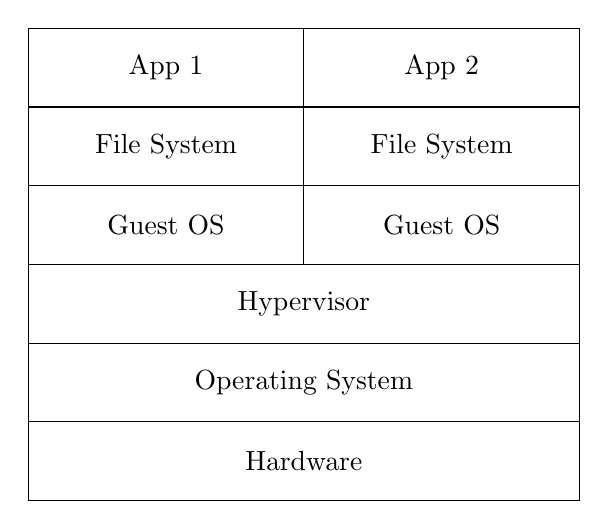
\begin{tikzpicture}[every fit/.style={inner sep=0pt, outer sep=0pt, draw}]
    \begin{scope}[y=1cm]
        \node [fit={(0,0) (7,1)}, label=center:{Hardware}] {};
    \end{scope}

    \begin{scope}[yshift=1cm,y=1cm]
        \node [fit={(0,0) (7,1)}, label=center:{Operating System}] {};
    \end{scope}

    \begin{scope}[yshift=2cm,y=1cm]
        \node [fit={(0,0) (7,1)}, label=center:{Hypervisor}] {};
    \end{scope}

    \begin{scope}[yshift=3cm,y=1cm]
        \node [fit={(0,0) (3.5,1)}, label=center:{Guest OS}] {};
        \node [fit={(3.5,0) (7,1)}, label=center:{Guest OS}] {};
    \end{scope}

    \begin{scope}[yshift=4cm,y=1cm]
        \node [fit={(0,0) (3.5,1)}, label=center:{File System}] {};
        \node [fit={(3.5,0) (7,1)}, label=center:{File System}] {};
    \end{scope}

    \begin{scope}[yshift=5cm,y=1cm]
        \node [fit={(0,0) (3.5,1)}, label=center:{App 1}] {};
        \node [fit={(3.5,0) (7,1)}, label=center:{App 2}] {};
    \end{scope}
    
\end{tikzpicture}
\caption{Two virtual machines running on a host}
\end{subfigure}
\hfill
\begin{subfigure}[b]{0.45\textwidth}
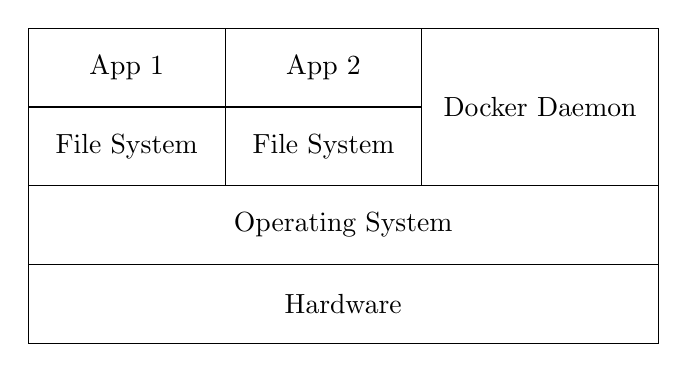
\begin{tikzpicture}[every fit/.style={inner sep=0pt, outer sep=0pt, draw}]
    \begin{scope}[y=1cm]
    \node [fit={(0,0) (8,1)}, label=center:{Hardware}] {};
    \end{scope}

    \begin{scope}[yshift=1cm,y=1cm]
        \node [fit={(0,0) (8,1)}, label=center:{Operating System}] {};
    \end{scope}
    
    \begin{scope}[yshift=2cm,y=2cm]
    \node [fit={(0,0) (2.5,0.5)}, label=center:{File System}] {};
    \node [fit={(0,0.5) (2.5,1)}, label=center:{App 1}] {};
    \node [fit={(2.5,0) (5,0.5)}, label=center:{File System}] {};
    \node [fit={(2.5,0.5) (5,1)}, label=center:{App 2}] {};
    \node [fit={(5,0) (8,1)}, label=center:{Docker Daemon}] {};
    \end{scope}
\end{tikzpicture}
\caption{Two containers running on a host}
\end{subfigure}

\caption{Comparison of virtual machines and containers}
\end{figure}

Unlike virtual machines, containers do not run on virtual hardware,
instead, containers run on the operating system of the host machine.
The obvious advantage of this is containers run much more efficiently than virtual machines.
Containers however, manage to remain isolated and it is at this point that we should explain how docker actually works.
Docker is built upon two individually fascinating technologies; namespaces, and layered filesystems.

\subsection{Namespaces}
The first technology, namespaces, is built into the linux kernel.
Linux namespaces were first introduced into the kernel in 2002, inspired by the concept introduced by the Plan 9 operating system from Bell Labs in the 1980s.
Namespaces enable the partitioning and thus, isolation, of various concepts managed and maintained by an operating system.
Initially namespaces were implemented to allow isolated filesystems (the so-called `mount' namespace).
Eventually, as namespaces were expanded to include process isolation, network isolation, and user isolation,
the ability to mimic an entirely new isolated machine was realised; containers were born%
.\footnote{Of course, containers in a rudamentry form existed before introduction to the linux kernel but we have to start somewhere. \url{https://blog.aquasec.com/a-brief-history-of-containers-from-1970s-chroot-to-docker-2016}}

Namespaces provide a mechanism to create an isolated environment within your current OS.
The creation of such an isolated environment with namespaces has been made quite easy --- you can create an isolated namespace with just a series of bash commands.
Niklas Dz{\"o}sch's talk `docker without docker', uses just 84 lines of Go code (which docker itself is written in),
to create, well, docker without docker.\footnote{\url{https://www.youtube.com/watch?v=7H__eF6hvWg}}
But namespaces are just the first technology which enables docker.
How do you pre-populate these isolated environments with everything you need to run a program?
To see what's in the isolated environment, we would run \texttt{ls} which, oh, requires the \texttt{ls} binary.
Furthermore, to even consider running a command we need a shell to type it in, so, oh, we should also have a \texttt{bash} binary.
And so on until, oh, finally, we have a linux kernel at least%
!\footnote{You might be asking yourself, wait but I have a Windows operating system and I can still run docker, what gives? The answer, ironically enough, a virtual machine!}

\subsection{Layered Filesystem}
A core principle of unix operating systems is that everything is a file.
Naturally then, if we want to start using a isolated environment,
all we need to do is copy in all the files which together form an operating system, right?
Well, yes, kind of.
In principle this is all you need do but this would hardly enable the popularity docker enjoys today.

Say that you want to send your coworker a docker container which has nginx (a tool for routing web traffic)
setup in just the way you need to pass incoming traffic to various components of your application.
Let's assume that you've setup nginx in ubuntu.
All you would need to do is zip up all the files which compose the ubuntu OS (an impressively small 188MB)
then all the files installed by nginx (about 55MB) and finally all the configuration files which you have modified,
somewhere in the order of 1000 bytes or 1 KB.
In total you're sending your coworker about 243MBs worth of data, less than a gigabyte, so they aren't too upset.

Now once we've finished developing our application and we're ready to package it up and send it to the world.
Rather than trying to support every known OS, we bundle all our services in docker containers,
one for nginx, one for mysql, one for our web application, etc, etc.
If your applications containers are as popular as nginx, this means one \textsl{billion} downloads of your container.
At a size of 243MBs, you've contributed 243 \textsl{petabytes} to the worlds collective bandwidth usage, and that's just your nginx container.

Dockers success over other containerization applications comes from the way it avoids this looming data disaster.
A concept known as the layered, or overlayed, or the stacked filesystem solves the problem.
First proposed in the early 1990s, layered filesystems enable layers of immutable files to be stacked below a top-level writable system.
This has the effect of producing a seemingly mutable (or writable) filesystem while never actually modifying the collection of immutable files.
Whenever a immutable file is `written to', a copy of the file is made and all modifications are written to this file.
When reading or listing files, the filesystem overlays the layers of immutable files together with the layer of mutable files.
This gives the appearance of one homogeneous filesystem.

Docker uses this technique to reduce the amount of duplicated files.
If you have docker containers which run nginx, mysql, and python but all containers run on ubuntu,
then your computer will only need to store one copy of the ubuntu filesystem.
Each container will store the changes to the base OS required to install each application and project that layer over the immutable ubuntu filesystem.

\subsection{Summary}
While docker itself only came out in 2013, the two primary technologies which it is composed of; namespaces, and the layered filesystem;
were around since the early 1990s.
Docker combines these technologies to enable applications to run in an isolated environment which can be efficiently replicated across different host computers.
The reproducablity of docker containers and the fact that they are so light weight makes them an ideal target for two important aspects of modern development;
developers simulating production environments locally, and duplicating production machines to scale for large loads of traffic.


\section{Docker FROM scratch}
Now that we understand the fundamentals of how docker works, let's start building our very first docker container.
To follow along, you will need to have docker installed on your
computer\footnote{\url{https://docs.docker.com/get-docker/}} and have access to basic unix command line
applications.\footnote{For windows users, I would recommend Windows Subsystem for Linux}

To start with, we'll write a \texttt{Dockerfile} which builds a docker image without an operating system and just prints `Hello World'
\cite{docker-from-scratch}.
The docker `code' is written in a \texttt{Dockerfile} which is then `compiled' into a docker image and finally run as a docker container.
The first command in your \texttt{Dockerfile} should always be \texttt{FROM}.
This command tells docker what immutable filesystem we want to start from, often, this will be your chosen operating environment.
In this exercise, since we don't want an operating system, we start with \texttt{FROM scratch},
a no-op instruction that tells docker to start with an empty filesystem.

Let's get something in this container.
For this, we'll use the \texttt{COPY} command which copies files from the host machine (your computer) into the container.
For now, we'll write \texttt{COPY hello-world /}, which says to copy a file from the current directory named \texttt{hello-world} into the root directory (\texttt{/})
of the container.
We don't yet have a \texttt{hello-world} file but we can worry about that later.
Finally, we use the \texttt{CMD} command to tell the container what to do when it is run.
This should be the command which starts your application.

\begin{shaded*}
\lstinputlisting[language=docker]{from-scratch/Dockerfile}
\end{shaded*}


Next, we'll need a minimal hello world program.
Unfortunately, we'll have to use C here as better programming languages have a bit too much overhead.
For everyone who has done CSSE2310, this should be painfully familiar, create a \texttt{main} function, print hello world, with a new line, and return 0.

\begin{shaded*}
\lstinputlisting[language=C,style=clang]{from-scratch/hello-world.c}
\end{shaded*}

Let's try running this container.\hint{Try to guess if this is going to work, why? why not?}

First, the hello world program needs to be compiled into a binary file.

\begin{shaded*}
\begin{lstlisting}[language=shell]
    >> gcc -o hello-world hello-world.c
    >> ls
    Dockerfile      hello-world     hello-world.c
\end{lstlisting}
\end{shaded*}

Next we'll use the \texttt{Dockerfile} to build a docker image and run that image.
Images are stored centrally for a user account so to identify the image, we need to tag it when it is built, we'll use `hello'.

\begin{shaded*}
\begin{lstlisting}[language=shell]
    >> docker build --tag hello .
    >> docker run hello
    standard_init_linux.go:228: exec user process caused: no such file or directory
\end{lstlisting}
\end{shaded*}

Unless this is dockers unique way of saying hello world, something has gone terribly wrong.
Here we're illustrating the power of docker isolation as well as the difficulty of not having an operating system.
This very simple hello world program still relies on other libraries in the OS, libraries which aren't available in the empty docker container.
\texttt{ldd} tells us exactly what \texttt{hello-world} depends on.
The hello world program can be statically compiled so that it doesn't depend on any libraries \cite{static-hello-world}.

\begin{shaded*}
\begin{lstlisting}[language=shell]
    >> ldd hello-world
        linux-vdso.so.1 (0x00007ffc51db1000)
        libc.so.6 => /lib/x86_64-linux-gnu/libc.so.6 (0x00007fcff8553000)
        /lib64/ld-linux-x86-64.so.2 (0x00007fcff8759000)
    >> gcc -o hello-world hello-world.c -static
    >> ldd hello-world
        not a dynamic executable
    >> docker build --tag hello .
    >> docker run hello
    Hello World
\end{lstlisting}
\end{shaded*}

Now we have a docker image built from scratch, without an operating system, which can say `Hello World'!
\begin{extra}
If you're interested in exploring in more depth, try using the `\texttt{docker image inspect hello}'
and `\texttt{docker history hello}' commands.
\end{extra}


\bibliographystyle{plain}
\bibliography{articles}

\end{document}